% Template for ASRU-2015 paper; to be used with:
%          spconf.sty  - ICASSP/ICIP LaTeX style file, and
%          IEEEbib.bst - IEEE bibliography style file.
% --------------------------------------------------------------------------
\documentclass{article}
\usepackage{spconf,amsmath,graphicx}
\usepackage{multirow}
\usepackage{caption,subcaption}
\usepackage{url}

% Example definitions.
% --------------------
\def\x{{\mathbf x}}
\def\L{{\cal L}}

% TODO, remove this later
\usepackage{xcolor}
\newcommand\davidnote[1]{\textcolor{red}{#1}}
% Remove later ^


% Title.
% ------
\title{Time delay deep neural network-based universal background models for speaker recognition}
%
% Single address.
% ---------------
\name{David Snyder, Daniel Garcia-Romero, Daniel Povey\thanks{This material is based upon work supported by the National Science Foundation Graduate Research Fellowship under Grant No. 1232825. Any opinion, findings, and conclusions or recommendations expressed in this material are those of the authors(s) and do not necessarily reflect the views of the National Science Foundation.}}
\address{Center for Language and Speech Processing \& Human Language Technology Center of Excellence\\
The Johns Hopkins University, Baltimore, MD 21218, USA\\
{\small \tt david.ryan.snyder@gmail.com, dgromero@jhu.edu, dpovey@gmail.com}}
%
% For example:
% ------------
%\address{School\\
%	Department\\
%	Address}
%
% Two addresses (uncomment and modify for two-address case).
% ----------------------------------------------------------
%\twoauthors
%  {A. Author-one, B. Author-two\sthanks{Thanks to XYZ agency for funding.}}
%	{School A-B\\
%	Department A-B\\
%	Address A-B}
%  {C. Author-three, D. Author-four\sthanks{The fourth author performed the work
%	while at ...}}
%	{School C-D\\
%	Department C-D\\
%	Address C-D}
%
\begin{document}
%\ninept
%
\maketitle
%
\begin{abstract}

Recently, deep neural networks (DNN) have been incorporated into i-vector-based speaker
recognition systems, where they have achieved state-of-the-art performance. In these
systems, a DNN replaces the Gaussian mixture model (GMM) as the universal background
model (UBM). In this study the DNN is a recently developed time delay deep neural network
(TDNN) that has achieved promising results in LVCSR tasks. 
We believe that the
TDNN-based system achieves the best reported results on SRE10 and it obtains a 50\% relative 
improvement over our GMM baseline in terms of equal error rate (EER). 
For some applications the computational cost of a DNN is prohibitive. 
Therefore we also investigate a lightweight alternative in which a supervised GMM is derived from
the TDNN posteriors. This method maintains the speed of the traditional unsupervised-GMM
but achieves a 20\% relative improvement in EER.
\end{abstract}
%
\begin{keywords}
speaker recognition, deep neural networks, time delay neural networks
\end{keywords}
%
\section{Introduction}
\label{sec:intro}

Modern speaker recogntion systems are based on i-vectors \cite{ivector}.
In this paradigm, a universal background model (UBM) is used to collect
sufficient statistics for i-vector extraction and a probabilistic 
linear discriminant analysis (PLDA) backend computes a similarity score between i-vectors
 \cite{plda_prince, brummer2010speaker, kenny2010bayesian, villalba2011towards, garcia2011analysis, garcia2012multicondition}.

Recent speaker recognition systems have improved performance by replacing 
the GMM-based UBM with a DNN \cite{lei2014, garcia2014}. 
Usually a DNN trained as the acoustic model in
an automatic speech recognition (ASR) system is repurposed for
speaker recognition, where it assumes the role of the UBM.
The output layer of a DNN provides soft alignments for
phonetic content, often tied triphone states (or senones). 
The DNN posteriors are used in conjunction with features extracted using a 
standard approach for speaker recognition, to create sufficient statistics
for i-vector extraction \cite{ivector}.
The advantage of the DNN over the GMM may
be due to its ability to directly model phonetic content, rather than an arbitrary
acoustic space \cite{lei2014, garcia2014, kenny2014deep}. In \cite{garcia2014} it was found that
improvements to DNNs in terms of ASR word error rate (WER) may translate into 
improvements in speaker
recognition performance. Recently, recurrent neural networks (RNN) and TDNNs \cite{tdnn} have
outperformed traditional DNNs for a variety of LVCSR tasks \cite{lstm, saon2014, multisplice}.
In particular, the multisplice TDNN \cite{multisplice} had an 11\% WER
on Switchboard, better than RNN systems on the same task.
Our DNN is based on \cite{multisplice}. 

The DNN-based speaker recognition methods achieve excellent results, but the
performance comes at the cost of increased computational complexity. During
i-vector extraction, the role of the UBM is to produce frame-level posteriors.
For a DNN, the computation is nontrivial. In a resource limited application
that nonetheless requires realtime performance, the DNN-based system may
be impractical. Ideally, a supervised-GMM could be created with the 
speed of the traditional GMM-based UBM but with heightened phonetic awareness.
In \cite{omar2010} a GMM-based ASR acoustic model replaced the usual GMM-UBM
to create a phonetically aware GMM, but the improvements were only consistent
during model combination \cite{omar2010}.

Usually DNN-based speaker recognition systems employ a supervised-GMM
derived from the DNN posteriors and speaker recognition features (often
not the same as the DNN features) \cite{lei2014, garcia2014, kenny2014deep}.
However, this GMM is not typically
used as a UBM; it has a minor role during i-vector extractor training.
Promoting this supervised GMM to the role of the UBM was explored
in \cite{lei2014}, but it did not improve on their baseline.
It was speculated that this is due
to the GMM's limited ability to model phonetic information. However,
that supervised GMM was diagonal, which possibly
reduced its modeling capacity. In this paper we reexamine the 
value of this supervised-GMM as a lightweight alternative to the DNN-based
speaker recognition system, and find that it consistently outperforms the
baseline.

\section{Experimental Setup}

\subsection{Datasets}
\label{datasets}
We evaluate our systems on the condition 5 extended task of 
SRE10 \cite{sre10}. The test consists of conversational telephone speech
in enrollment and test utterances. In total there are 416,119 trials,
over 98\% of which are nontarget comparisons. 

The UBM and i-vector extractor training data consists of male and female
utterances from SWB and NIST SREs prior to 2010. The SWB data contains
1,962 speakers and 20,905 utterances of SWB Cellular and SWB 2 
Phases II and III. The SRE dataset consists of 3,805 speakers 
and 36,614 utterances.
The PLDA backend is trained only on the SRE data. About 1,800 hours
of the english portion of Fisher \cite{fisher} is
used to train the TDNN.

\subsection{DNN Recipe}
\label{dnn_recipe}

The system is a 6-layer deep neural network based on the multisplice 
time delay DNN described
in \cite{multisplice}. This architecture is currently the recommended
recipe in the Kaldi toolkit \cite{kaldi} for large-scale speech recognition. 
In the multisplice system, a narrow temporal
context is provided to the first layer and increasingly large temporal
contexts are available to the subsequent hidden layers. The result is that
higher levels of the network are able to learn greater temporal
relationships. 

The features are 40 MFCCs (without cepstral
truncation) with 25ms frames. Cepstral mean subtraction is 
performed over a window of
6 seconds. Five frames are spliced together at the
input layer and an increasingly wide context is provided to 
subsequent hidden layers. The hidden layers use the $p$-norm (where $p=2$)
activation function \cite{pnorm}. 
To facilitate faster computation, the size of the network is reduced
from what is described in \cite{multisplice}. The hidden layers have an 
input dimension of 350 and an output dimension 3500. 
The softmax output layer computes posteriors for 5297 triphone states. No
fMLLR or i-vectors are used for speaker adaptation.

\subsection{GMM-UBM Baseline}
\label{gmm_sys}

\begin{figure}[th]
\centerline{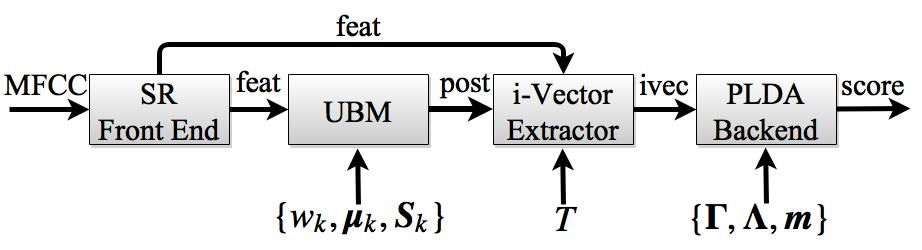
\includegraphics[width=8.5cm]{fig/baseline_schema}}
\caption{GMM-based speaker recognition schema.}
\label{fig:gmm_schema}
\end{figure}

The UBM in our baseline system illustrated in Figure \ref{fig:gmm_schema} 
is a full-covariance
GMM with several thousand mixture components. We compare systems with
2048, 4096, and 5297 components. The front-end consists of 20 MFCCs which
are mean normalized over a 3 second window, plus $\Delta$ 
and $\Delta \Delta$ to create a 60 dimension frame-level feature vector.
The nonspeech frames are then eliminated using
energy-based Voice Activity Detection (VAD). The GMM is trained on SWB
and the SRE datasets. The 
full-covariance GMM is initially a diagonal
covariance GMM which is trained for 4 iterations of EM followed by
an additional 4 iterations using a full-covariance matrix.
 A 600 dimensional i-vector extractor is also trained on 
SWB + SRE for 5 iterations of EM. In Figure \ref{fig:gmm_schema} the PLDA
backend also includes the i-vector mean $\boldsymbol{m}$ subtraction and
length normalization. The between-class and within-class
covariance matrices $\boldsymbol{\Gamma}$ and $\boldsymbol{\Lambda}$ of the PLDA backened along with
the vector $\boldsymbol{m}$ are trained on the SRE dataset described 
in Section \ref{datasets}.

\subsection{Supervised GMM-UBM}
\label{sup_gmm_sys}

To create the supervised-GMM, DNN posteriors from the system in Section \ref{dnn_recipe}
and speaker recognition
features described in Section \ref{gmm_sys} are computed on the training data (SWB + SRE)
 using the
equations in \ref{eq:sup_gmm_eq}. The DNN parameters are collectively
labeled $\boldsymbol{\Theta}$ and 
$Pr(k \mid \boldsymbol{y}_{i}, \boldsymbol{\Theta})$ is the
probability of senone $k$ given the DNN features $\boldsymbol{y}_{i}$. The
corresponding speaker recognition features are denoted $\boldsymbol{x}_{i}$.
In contrast to \cite{lei2014}, our supervised-GMM is full-covariance.

\begin{equation}
\label{eq:sup_gmm_eq} 
\begin{split}
z_{k}^{(i)} &= Pr(k \mid \boldsymbol{y}_{i}, \boldsymbol{\Theta}), \\
w_{k} &= \sum_{i=1}^{N}z_{k}^{(i)},\\
\boldsymbol{\mu}_{k} &= \frac{1}{w_{k}} \sum_{i=1}^{N} z_{k}^{(i)} \boldsymbol{x}_{i},\\
\boldsymbol{S}_{k} &= \frac{1}{w_{k}} \sum_{i=1}^{N} z_{k}^{(i)} (\boldsymbol{x}_{i} - \boldsymbol{\mu}_{k}) (\boldsymbol{x}_{i} - \boldsymbol{\mu}_{k})^{\top}.
\end{split}
\end{equation}

Since the DNN output layer has 5297 senones, the supervised GMM also has 5297
components. The supervised and unsupervised GMMs differ only
in the UBM training proceedure. Training of the $\boldsymbol{T}$ matrix
and PLDA parameters $\boldsymbol{\Gamma}$ and $\boldsymbol{\Lambda}$ are unchanged from Section \ref{gmm_sys}.

\subsection{TDNN-UBM}

\begin{figure}[th]
\centerline{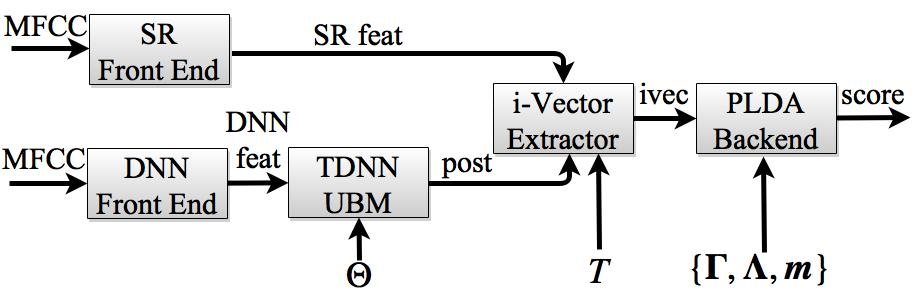
\includegraphics[width=8.5cm]{fig/dnn_schema}}
\caption{TDNN-based speaker recognition schema.}
\label{fig:dnn_schema}
\end{figure}

The TDNN system uses the supervised-GMM described in 
section \ref{sup_gmm_sys} to initialize the i-vector 
extractor $\boldsymbol{T}$ matrix.
However, updating the $\boldsymbol{T}$ matrix and extracting 
i-vectors uses DNN posteriors and 
speaker recognition features. As in Sections \ref{gmm_sys} and \ref{sup_gmm_sys},
 the i-vectors are 600 dimensional and the PLDA backend is the same.

In order to maintain the correct temporal context for the DNN, VAD
is not used at the frontend. Instead, the voice activity detection from the speaker recognition
features are reused to filter the posteriors of the network.

\subsection{System Design}
Experiments used ASR and speaker recognition modules in the
Kaldi speech recognition toolkit \cite{kaldi}. The recipes are
available in in the Kaldi code repository.

\section{RESULTS}
\begin{table}
\begin{center}
\begin{tabular}{l|ccc}
\hline
System & EER(\%) & DCF$10^{-3}$ & DCF$10^{-2}$ \\ \hline \hline
Sup-GMM-5297 & 1.94 & 0.388 & 0.213 \\
TDNN-5297 & 1.20 & 0.216 & 0.123 \\
GMM-2048 & 2.49 & 0.496 & 0.288 \\
GMM-4096 & 2.56 & 0.468 & 0.287 \\
GMM-5297 & 2.42 & 0.484 & 0.290 \\ \hline
\end{tabular}
\end{center}
\caption{Performance comparison of gender independent models on SRE10 C5.}
\label{gender_ind}
\end{table}

\begin{table}
\begin{center}
\begin{tabular}{l|ccc}
\hline
System & EER(\%) & DCF$10^{-3}$ & DCF$10^{-2}$ \\ \hline \hline
Sup-GMM-5297 & 1.65 & 0.354 & 0.193 \\
TDNN-5297 & 1.09 & 0.214 & 0.108 \\
GMM-2048 & 2.16 & 0.417 & 0.239 \\
GMM-4096 & 1.96 & 0.414 & 0.227 \\
GMM-5297 & 2.00 & 0.410 & 0.241 \\ \hline
\end{tabular}
\end{center}
\caption{Performance comparison of gender dependent models on SRE10 C5.}
\label{gender_dep}
\end{table}

\begin{figure}[t]
\centerline{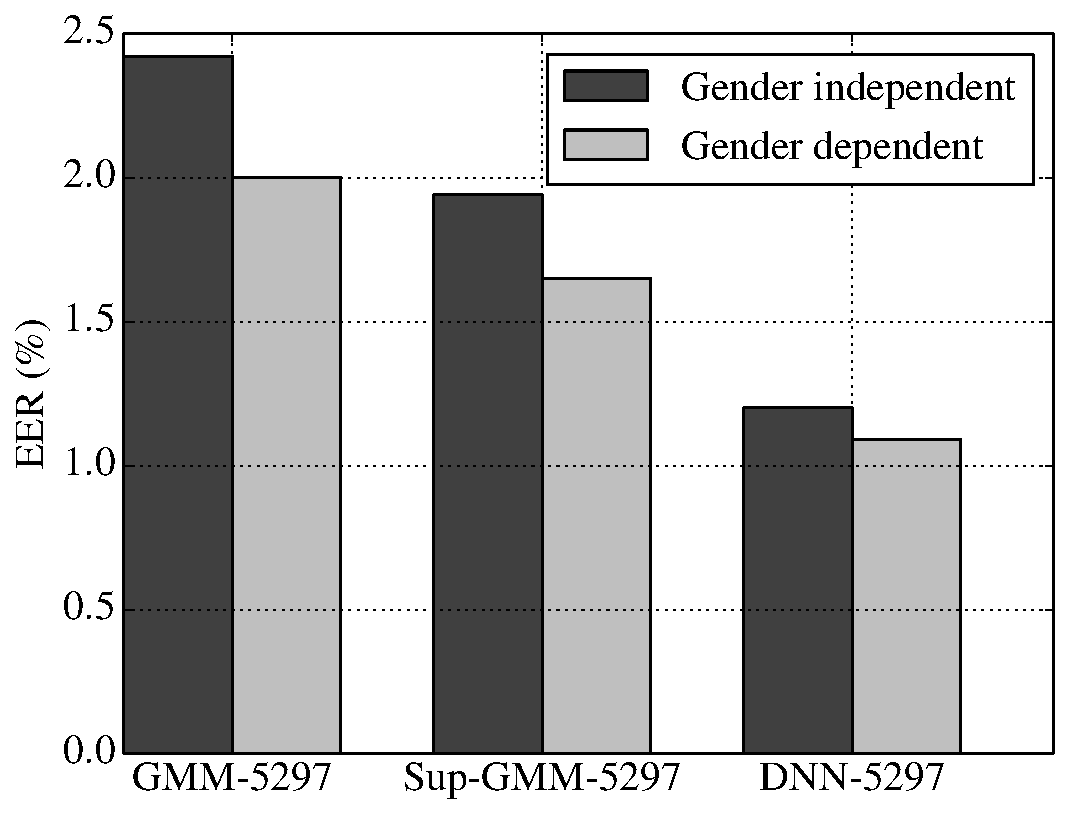
\includegraphics[width=8.5cm]{fig/eer}}
\caption{Comparison of EERs.}
\label{fig:eer}
\end{figure}

\begin{figure}[t]
\centerline{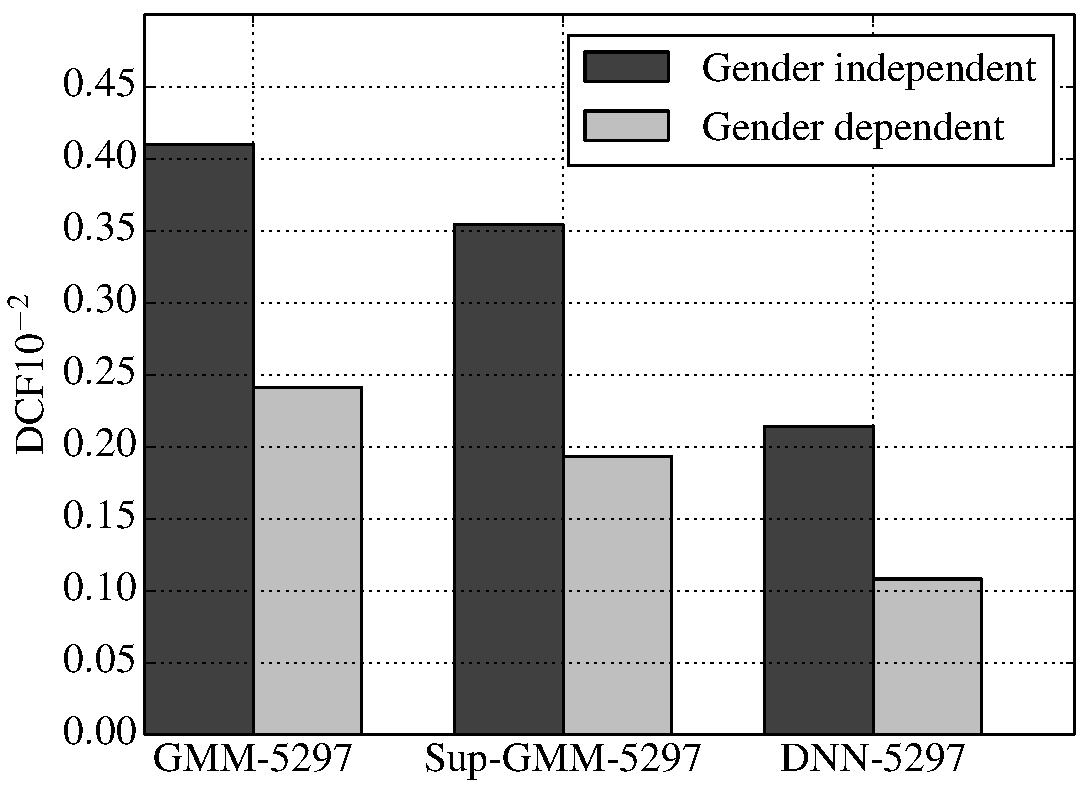
\includegraphics[width=8.5cm]{fig/dcf-2}}
\caption{Comparison of DCF$10^{-2}$.}
\label{fig:dcf_2}
\end{figure}

\begin{figure}[t]
\centerline{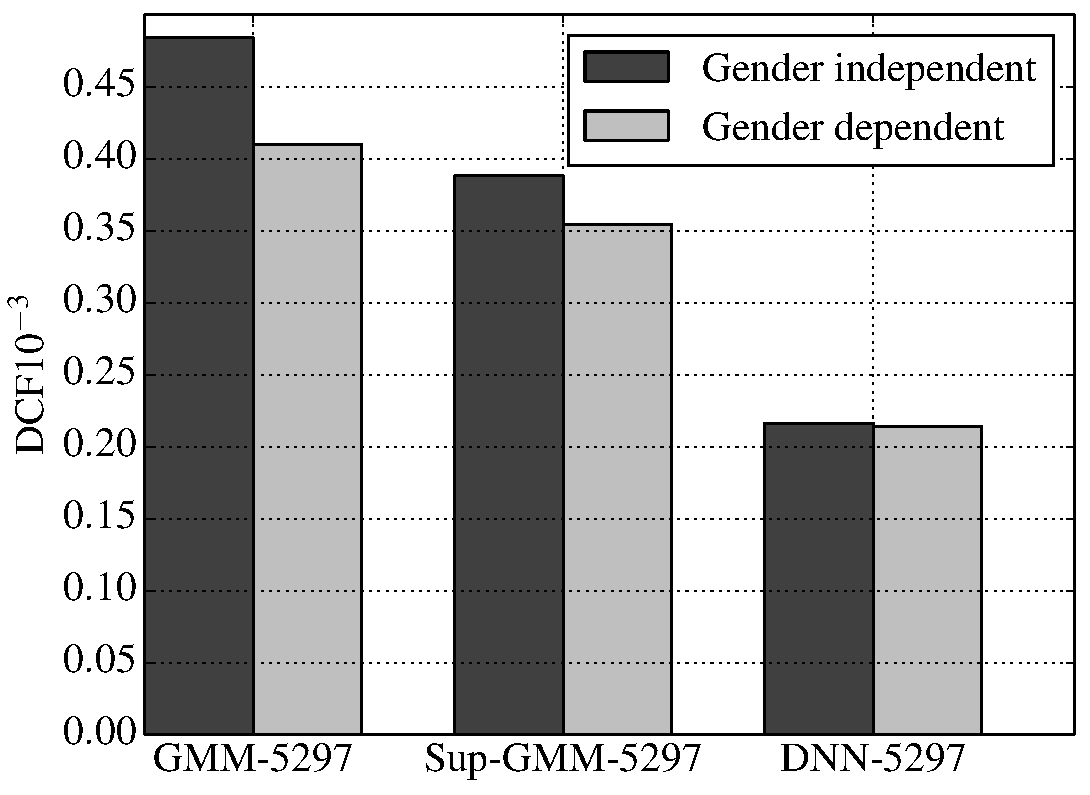
\includegraphics[width=8.5cm]{fig/dcf-3}}
\caption{Comparison of DCF$10^{-3}$.}
\label{fig:dcf_3}
\end{figure}

\begin{figure}[th]
\centerline{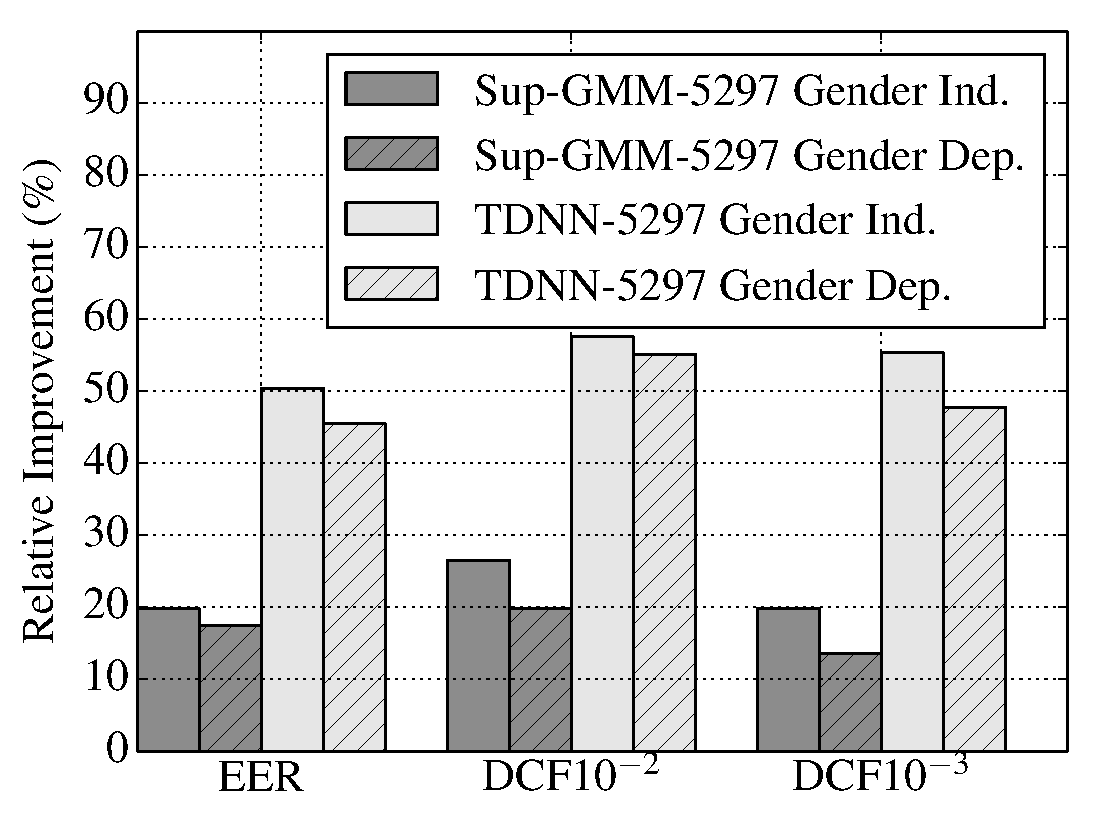
\includegraphics[width=8.5cm]{fig/rel}}
\caption{Relative improvement over
              the GMM-5297 baseline.}
\label{fig:rel}
\end{figure}

We compare gender independent and gender dependent versions of the
baseline GMM, sup-GMM and TDNN systems. The gender independent
systems each have a single pipeline which evaluates all of the SRE10
extended condition 5. The gender dependent systems share most of the
same components with the gender independent systems. 
The SRE data is partitioned into male and female sets and two PLDA
backends are trained. Accordingly, we evaluate the gender
dependent models on just the male or female portions of SRE10. To avoid 
overly large
tables we only report the performance for pooled gender dependent
and independent scores.

In Tables \ref{gender_ind} and \ref{gender_dep} we see that there
isn't much of a performance difference between
the unsupervised GMMs with 2048, 4096 and 5297 components. 
We choose GMM-5297 as our primary baseline, since it has, by a small margin,
the highest gender independent results of the baseline models.

Figures \ref{fig:eer}, \ref{fig:dcf_2}, and \ref{fig:dcf_3}
compare the performance among the GMM-5297,
sup-GMM-5297 and TDNN-5297 systems. The DNN-based systems achieve the
best results, with TDNN-5297 obtaining 1.20\% and 1.09\%
gender independent and gender dependent EERs respectively.
Figure \ref{fig:rel} illustrates the relative improvement of the
TDNN and sup-GMM over the GMM-5297 baseline. Across the three
operating points on the gender indendent and dependent systems we 
see a relative improvement of 13.65\%-26.55\%
by the sup-GMM and 47.80\%-57.59\% by the TDNN. Although
the performance of the sup-GMM is less than the TDNN,
it nevertheless outperforms the baseline by a significant
margin. In similar methods such as \cite{lei2014} and \cite{omar2010}
the supervised-GMM did not result in a significant improvement by
itself. Perhaps the underlying reason lies in the overall quality of
the TDNN which the sup-GMM is based on. Additionally, 
full-covariance may allow the sup-GMM to retain modeling capacity.

\begin{figure}[t]
\centerline{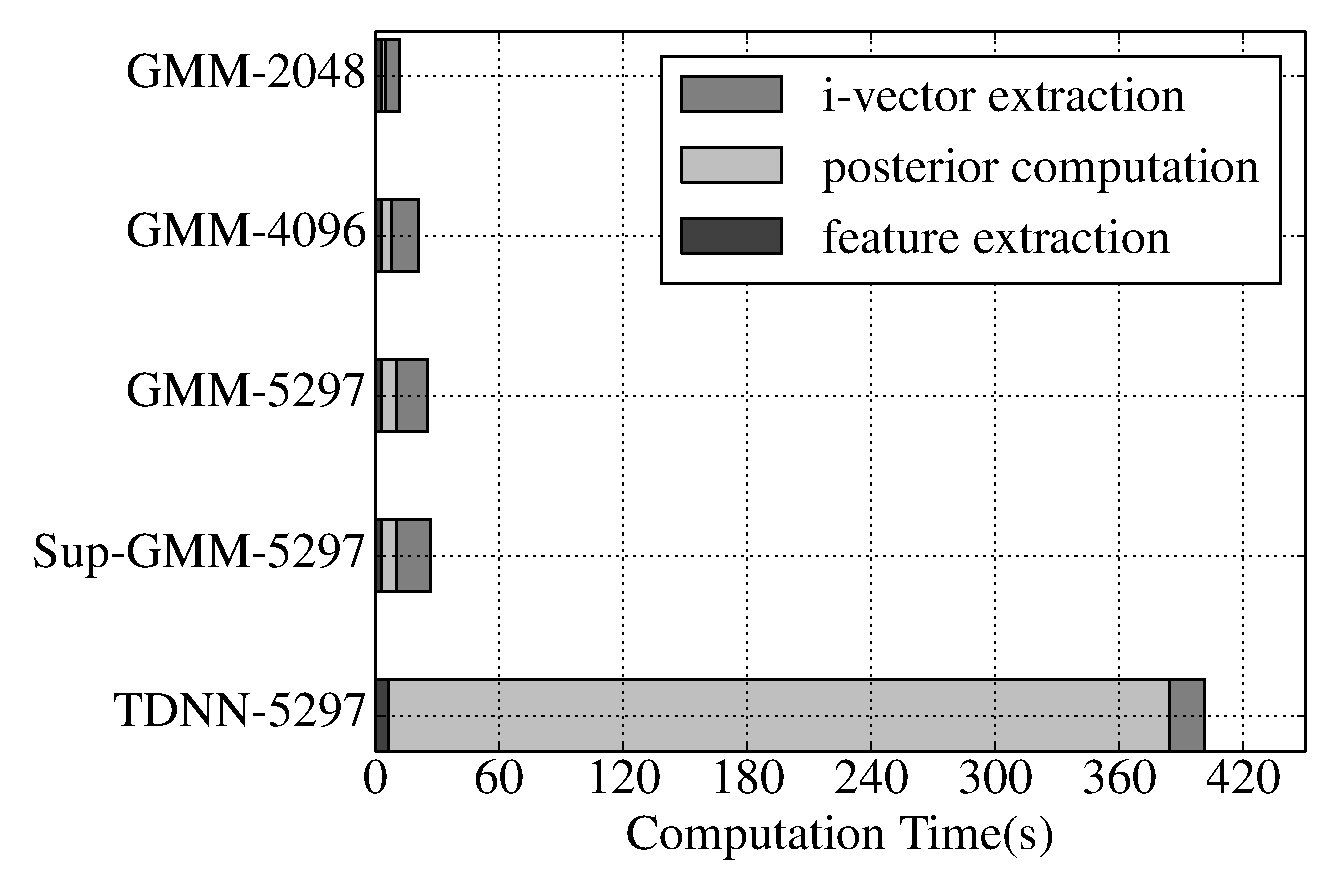
\includegraphics[width=8.5cm]{fig/time}}
\caption{CPU time relative to utterance length for each system.}
\label{fig:time}
\end{figure}

The primary advantage of a GMM-based method lies in its
efficiency during i-vector extraction. Using the sum of the \texttt{usr}
and \texttt{sys}
portions of the Linux tool \texttt{time} we recorded the duration of
different parts of the system pipelines. In Table \ref{timing} and
Figure \ref{fig:time} we represent this in terms of real-time factors.
Ten 5 minute utterances
were selected at random from the SRE10 test data and these were processed
and timed from feacture extraction to i-vector extraction 30 times. The
experiment was performed on an Intel x86-64 machine with 48 2000Mhz CPUs.
The real-time factors were obtained by taking the average durations In CPU and
dividing by the total utterance length. 

% TODO: Consider removing total. Note that the table is still too big
\begin{table}
\caption{CPU time relative to utterance length for primary stages of the system pipelines.}
\begin{center}
\begin{tabular}{l|cccc}
\hline
%System & Feat.(s) & Post.(s) & i-Vec.(s) & Tot.(s) \\ \hline \hline
%Sup-GMM-5297 & 3.05 & 10.39 & 16.32 & 29.76 \\
%TDNN-5297 & 6.46 & 384.05 & 17.30 & 407.81 \\
%GMM-5297 & 3.09  & 10.33 & 15.04 & 28.46 \\
%GMM-4096 & 3.04 & 8.00 & 12.82 & 23.86 \\
%GMM-2048 & 3.04 & 5.04 & 6.85 & 14.93 \\ \hline
System & Feat.(\%) & Post.(\%) & i-Vec.(\%) & Tot.(\%) \\ \hline \hline
Sup-GMM-5297 & 1.02 & 3.46 & 5.44 & 9.92 \\
TDNN-5297 & 2.15 & 128.02 & 5.77 & 135.94 \\
GMM-5297 & 1.03 & 3.44 & 5.01 & 9.49 \\
GMM-4096 & 1.01 & 2.67 & 4.27 & 7.95 \\
GMM-2048 & 1.01 & 1.68 & 2.28 & 4.98 \\ \hline
\end{tabular}
\end{center}
\label{timing}
\end{table}


The GMM-2048 system is about twice as fast as the
larger GMMs with 4096 or 5297 components during posterior and i-vector
extraction. Even without
parallelization the GMM-based systems are at least ten times faster than
real-time. Since the TDNN system needs to compute features for both the
DNN and for speaker recognition this stage of the pipeline is about twice
as slow as the GMM-based systems.
Without parallelization, the vast majority of the DNN-based system is spent 
in posterior calculation. This results in a system which is nearly 36\% slower 
than real-time, and more than ten times slower than the sup-GMM-5297.

In practice we would perform the DNN posterior matrix calculations in
CUDA to obtain faster than real-time performance.
However, by comparing the total CPU time between the systems, we
better expose the overall computational load of the DNN, and facilitate
a comparison of compute-cost vs. performance of the three systems. 


%\begin{figure*}[!t]
%\centering
%  \begin{subfigure}[b]{0.49\textwidth}
%  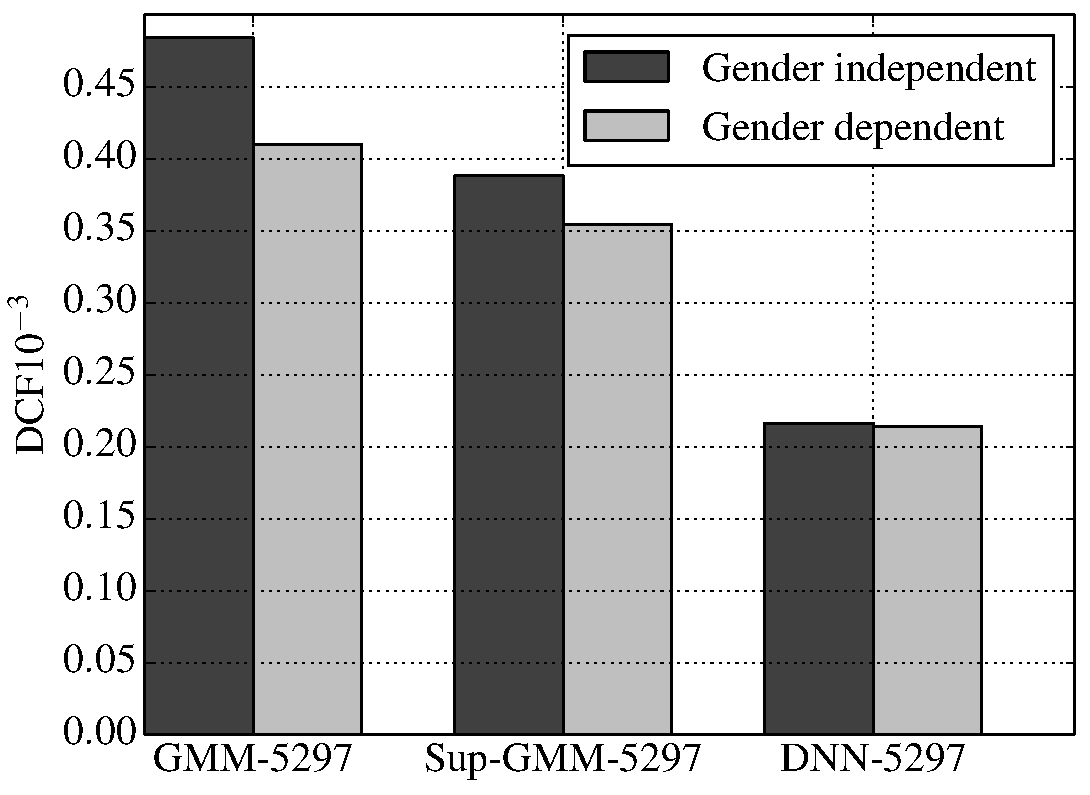
\includegraphics[width=8.5cm]{fig/dcf-3}     
%  \caption{}                           
%  \end{subfigure}
%  \begin{subfigure}[b]{0.49\textwidth}
%  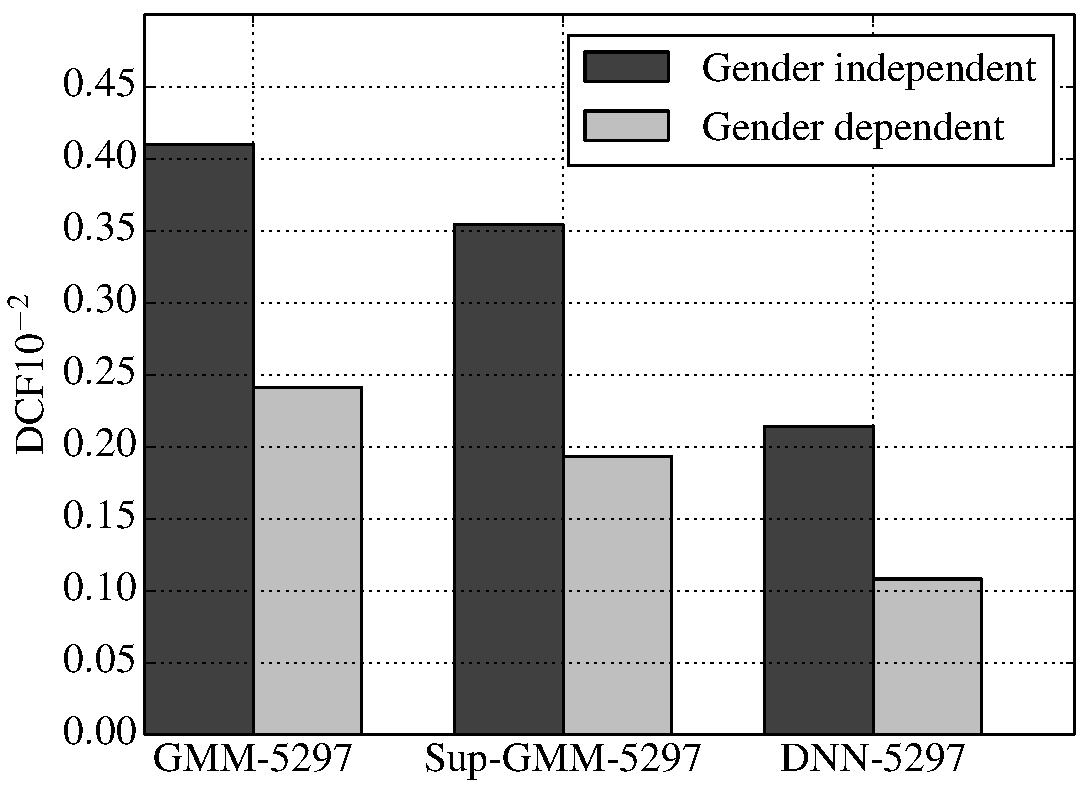
\includegraphics[width=8.5cm]{fig/dcf-2}   
%  \caption{}                                        
%  \end{subfigure}           
%  \caption{Performance on DCF with $10^{-3}$ and $10^{-2}$ operating points.}  
%  \label{fig:dcf}     
%\end{figure*}


%\begin{table}
%\begin{center}
%\begin{tabular}{l|ccc}
%\hline
%EER (\%) & Ind. Pool. & Ind. Fem. & Ind. Male \\ \hline \hline
%Sup-GMM & 1.94 & 1.98 & 1.79 \\
%DNN & 1.20 & 1.46 & 0.87 \\
%GMM-2048 & 2.49 & 2.35 & 2.51 \\
%GMM-4096 & 2.56 & 2.38 & 2.63 \\
%GMM-5297 & 2.42 & 2.43 & 2.40 \\ \hline
%\end{tabular}
%\end{center}
%\caption{EER on SRE10 C5 with gender independent models.}
%\label{eer_table}
%\end{table}
%
%\begin{table}
%\begin{center}
%\begin{tabular}{l|ccc}
%\hline
%EER (\%) & Dep. Pool. & Dep. Fem. & Dep. Male \\ \hline \hline
%Sup-GMM & 1.65 & 1.87 & 1.30 \\
%DNN & 1.09 & 1.43 & 0.72 \\
%GMM-2048 & 2.16 & 2.33 & 1.59 \\
%GMM-4096 & 1.96 & 2.14 & 1.41 \\
%GMM-5297 & 2.00 & 2.16 & 1.53 \\ \hline
%\end{tabular}
%\end{center}
%\caption{EER on SRE10 C5 with gender dependent models.}
%\label{eer_table}
%\end{table}

\section{Conclusion}

We explored the use of TDNNs for speaker recognition on the SRE10 task.
We found that this DNN yields a large relative improvement over the
unsupervised GMM baseline on EER and DCF operating points. With the
TDNN-UBM we also achieve a 1.20\% gender independent EER, 
which we believe is the best
reported on the task. We also highlighted the computational advantages
of the GMM over the DNN, and showed that there is a significant cost to
computing DNN posteriors. While GPU parallelization is commonly used to
obtain real-time performance, it may not be feasible for all applications.
We found that the supervised-GMM, normally
of minor use in the DNN-based system, can be 
used on its own as a fast alternative to the DNN with better performance
than the baseline. 

% References should be produced using the bibtex program from suitable
% BiBTeX files (here: strings, refs, manuals). The IEEEbib.bst bibliography
% style file from IEEE produces unsorted bibliography list.
% -------------------------------------------------------------------------
\bibliographystyle{IEEEbib}
\bibliography{refs}

\end{document}
